\documentclass[conference]{IEEEtran}

\usepackage[utf8]{inputenc}
\usepackage[spanish,es-nosectiondot]{babel}
\usepackage{cite}
\usepackage{graphicx}
\usepackage{amsmath,amssymb}
\usepackage{booktabs}
\usepackage{hyperref}

\graphicspath{{outputs/figures/}}

\renewcommand{\refname}{Referencias}

\begin{document}

\title{Clasificación Automática de Calidad de Frutas\\Mediante Visión por Computadora y Aprendizaje Automático}

\author{\IEEEauthorblockN{Nicolás Jiménez, Juan David Rosero}
\IEEEauthorblockA{Universidad ICESI\\
Facultad de Ingeniería, Diseño y Ciencias Aplicadas\\
Programa de Ingeniería de Sistemas --- APO III, Semestre 2026-1\\
\{nicolas.jimenez, juan.rosero\}@ejemplo.com}}

\maketitle

\begin{abstract}
Este trabajo presenta un sistema automático de clasificación de calidad de frutas basado en visión por computadora, utilizando el conjunto de datos \emph{Fruit Quality Classification} complementado con imágenes propias. Se entrenaron y evaluaron tres modelos supervisados: regresión logística, \emph{Random Forest} (RF) y una red neuronal convolucional (CNN). Los resultados muestran que tanto RF como CNN alcanzan una precisión superior al 96\,\% en datos de prueba, con un F1 \emph{macro} de 0.9615 y 0.9605 respectivamente. Se implementó una interfaz gráfica en Streamlit que permite cargar imágenes o capturarlas con la cámara y obtener la clasificación en tiempo real, junto con la cobertura de la fruta en el encuadre. El sistema aborda una necesidad real en el sector agroindustrial: la estandarización de la clasificación manual de productos frescos.
\end{abstract}

% ===========================================================================
% 3. INTRODUCCIÓN
% ===========================================================================
\section{Introducción}

\subsection{Contexto}
En mercados y agroindustrias, la clasificación manual de productos frescos según su calidad es un proceso lento, subjetivo y propenso a errores. Esta situación genera pérdidas económicas, desperdicio de alimentos y falta de estandarización en la cadena de suministro~\cite{kaggle_fruit}. La automatización de esta tarea mediante visión por computadora ofrece una solución reproducible, objetiva y escalable.

\subsection{Descripción del problema}
Se requiere un sistema capaz de analizar imágenes de frutas individuales sobre fondo simple y clasificarlas en tres categorías de calidad: \emph{bueno} (apto para consumo), \emph{regular} (defectos menores que requieren inspección adicional) y \emph{malo} (deterioro evidente, no comercializable). Adicionalmente, el sistema debe estimar la cobertura de la fruta en la imagen como medida de tamaño relativo.

\subsection{Justificación}
La estandarización de la clasificación de calidad tiene impacto económico directo: reduce el desperdicio al identificar oportunamente productos en mal estado, mejora la confianza del consumidor y permite a los productores optimizar sus procesos de empaque y distribución. La Organización de las Naciones Unidas para la Alimentación y la Agricultura (FAO) estima que aproximadamente un tercio de los alimentos producidos para consumo humano se pierde o desperdicia a nivel mundial~\cite{fao_waste}, y sistemas como el propuesto pueden contribuir a mitigar este problema.

% ===========================================================================
% 4. FUNDAMENTOS TEÓRICOS
% ===========================================================================
\section{Fundamentos teóricos}

\subsection{Extracción de características}
Para el enfoque de aprendizaje tradicional, las imágenes se redimensionan a 64\,$\times$\,64\,píxeles con relleno para preservar la relación de aspecto. Se extraen histogramas de color RGB (32 bins por canal) junto con la media y desviación estándar de cada canal, produciendo un vector de 102 características por imagen~\cite{histogram_features}.

\subsection{Random Forest}
Random Forest~\cite{breiman2001random} es un método de aprendizaje conjunto (\emph{ensemble learning}) basado en la combinación de múltiples árboles de decisión. Fue introducido por Leo Breiman en 2001 como una extensión del \emph{bagging} (Bootstrap Aggregating) que incorpora aleatoriedad tanto en los datos como en las características.

\subsubsection*{Fundamento: Bagging}
Cada árbol del bosque se entrena sobre una muestra bootstrap del conjunto original, es decir, una muestra con reemplazo del mismo tamaño que el conjunto de datos. Esto genera que aproximadamente el 63.2\,\% de las instancias originales aparezcan en cada muestra, mientras que el 36.8\,\% restante queda fuera (\emph{out-of-bag}, OOB) y puede usarse como conjunto de validación interno sin necesidad de dividir los datos~\cite{breiman1996bagging}. Al promediar las predicciones de árboles entrenados sobre diferentes subconjuntos, se reduce drásticamente la varianza sin incrementar el sesgo de manera significativa.

\subsubsection*{Aleatoriedad en las características}
Además del bootstrap, Random Forest introduce una segunda fuente de aleatoriedad: en cada nodo de cada árbol, solo se considera un subconjunto aleatorio de \(m\) características (donde \(m \ll M\), siendo \(M\) el total de características) para encontrar la mejor división. Esto garantiza que los árboles no estén correlacionados entre sí: si todos los árboles usaran las mismas características dominantes para dividir, el bosque sería esencialmente un solo árbol repetido. Con la aleatoriedad forzada, árboles diferentes aprenden patrones distintos, y la combinación de sus predicciones captura interacciones complejas que un solo árbol no podría modelar.

\subsubsection*{Mecanismo de decisión}
Para clasificación, cada árbol emite un voto por clase y el bosque selecciona la clase con más votos (votación mayoritaria). El resultado es un modelo robusto al ruido, resistente al sobreajuste (siempre que los árboles sean suficientemente profundos y numerosos), y capaz de modelar relaciones no lineales entre las características y las clases objetivo.

\subsubsection*{Ventajas para este problema}
Para nuestro conjunto de características de histogramas de color (102 dimensiones), Random Forest presenta ventajas decisivas frente a modelos lineales:
\begin{itemize}
  \item Captura interacciones no lineales entre bins de histograma (por ejemplo, cómo la relación entre el bin de rojo intenso y el bin de marrón indica podredumbre).
  \item No requiere normalización ni escalado de características.
  \item Proporciona una medida directa de importancia de cada característica, permitiendo interpretar qué aspectos cromáticos son más determinantes para la clasificación.
  \item El error OOB permite estimar el desempeño sin necesidad de un conjunto de validación separado.
\end{itemize}

\subsection{Redes neuronales convolucionales (CNN)}
Las CNN~\cite{lecun2015deep} son arquitecturas de \emph{deep learning} diseñadas para el procesamiento de datos con estructura de cuadrícula, como imágenes. Emplean capas de convolución para extraer patrones locales, capas de \emph{pooling} para reducir la dimensionalidad y capas densas para la clasificación final. La arquitectura implementada consta de tres capas convolucionales (32, 64 y 128 filtros) con normalización por lotes, \emph{max-pooling} y \emph{dropout} para regularización.

\subsection{Métricas de evaluación}
Las métricas empleadas son precisión (\emph{precision}), sensibilidad (\emph{recall}) y puntuación F1, definidas como:
\[
\text{Precision} = \frac{TP}{TP+FP},\quad
\text{Recall} = \frac{TP}{TP+FN},\quad
\text{F1} = 2\cdot\frac{\text{Precision}\cdot\text{Recall}}{\text{Precision}+\text{Recall}}.
\]
Dado el desbalanceo entre clases, se prioriza la métrica F1 \emph{macro} (media no ponderada del F1 de cada clase)~\cite{grandini2020metrics}.

% ===========================================================================
% 5. METODOLOGÍA
% ===========================================================================
\section{Metodología}

Se siguió la metodología CRISP-DM adaptada al proyecto:

\begin{enumerate}[leftmargin=*,nosep]
  \item \textbf{Comprensión del negocio:} Identificación del problema de clasificación manual y su impacto económico.
  \item \textbf{Comprensión de los datos:} Análisis exploratorio del conjunto \emph{Fruit Quality Classification} (27\,944 imágenes) y recolección de 30--50 imágenes adicionales por grupo.
  \item \textbf{Preparación:} Redimensionamiento, normalización, división 70/15/15 (train/val/test) y balanceo con SMOTE para la clase minoritaria (\emph{regular}).
  \item \textbf{Modelado:} Entrenamiento de tres modelos con búsqueda de hiperparámetros mediante \emph{GridSearch} con validación cruzada de 5 pliegues, maximizando F1 macro:\par
    \emph{Regresión logística:} regularización L2 con \(C \in \{0.1, 1.0, 10.0\}\) y \texttt{class\_weight="balanced"}.\par
    \emph{Random Forest:} búsqueda sobre 36 combinaciones: \texttt{n\_estimators} (100, 200, 300) controla la cantidad de árboles; \texttt{max\_depth} (None, 10, 20) limita la profundidad para evitar sobreajuste; \texttt{min\_samples\_split} (2, 5) define el mínimo de muestras para dividir un nodo; \texttt{max\_features} (\texttt{"sqrt"}, \texttt{"log2"}) controla la aleatoriedad en cada división. Se usó \texttt{class\_weight="balanced"} para compensar el desbalance.\par
    \emph{CNN:} 20 épocas, optimizador Adam (lr = 0.001), \emph{batch size} 32, \emph{early stopping} con paciencia de 5 épocas, aumentación de datos en tiempo real (volteo horizontal, rotación \(\pm 10^\circ\), contraste aleatorio).
  \item \textbf{Evaluación:} Comparación mediante F1 macro en validación; selección del mejor modelo para prueba final.
  \item \textbf{Despliegue:} Implementación de una aplicación web con Streamlit que permite subir imágenes o capturarlas con la cámara, obtener la clasificación y visualizar la cobertura de la fruta.
\end{enumerate}

\subsection{Datos}
El conjunto de datos \emph{Fruit Quality Classification}~\cite{kaggle_fruit} contiene 27\,944 imágenes distribuidas en 6 tipos de fruta (manzana, plátano, guayaba, lima, naranja, granada) y 3 clases de calidad. La Tabla~\ref{tab:distribucion} muestra la distribución.

\begin{table}[h]
\centering
\caption{Distribución de clases en el dataset.}
\label{tab:distribucion}
\begin{tabular}{lrr}
\toprule
Clase & Imágenes & Proporción \\
\midrule
Bueno  & 14\,307 & 51.2\,\% \\
Malo   &  9\,024 & 32.3\,\% \\
Regular&  4\,613 & 16.5\,\% \\
\midrule
Total  & 27\,944 & 100\,\% \\
\bottomrule
\end{tabular}
\end{table}

\begin{figure}[h]
\centering
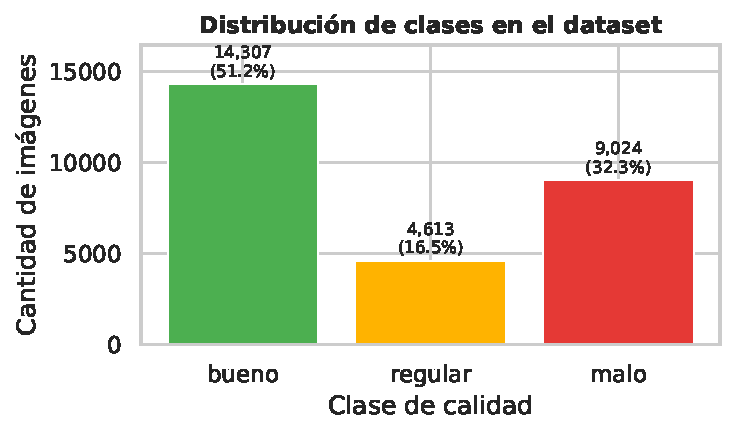
\includegraphics[width=\columnwidth]{fig_distribucion.pdf}
\caption{Distribución de imágenes por clase de calidad.}
\label{fig:distribucion}
\end{figure}

Se observa un desbalanceo significativo: la clase \emph{regular} es 3.1 veces menor que \emph{bueno}. Para mitigarlo, se aplicó SMOTE~\cite{chawla2002smote} sobre el conjunto de entrenamiento, balanceando las tres clases.

\subsection{Arquitectura de la CNN}
La CNN implementada consta de: entrada (64$\times$64$\times$3), Conv2D(32, 3$\times$3) + BatchNorm + ReLU + MaxPool(2$\times$2), Conv2D(64, 3$\times$3) + BatchNorm + ReLU + MaxPool(2$\times$2), Conv2D(128, 3$\times$3) + BatchNorm + ReLU + MaxPool(2$\times$2), Dropout(0.5), Dense(256, ReLU), Dropout(0.3) y Dense(3, Softmax).

\subsection{Estimación de cobertura}
Para estimar el tamaño relativo, se aplica detección de bordes mediante Canny~\cite{canny1986computational} seguido de cierre morfológico para obtener el contorno de la fruta. La cobertura se calcula como el área del rectángulo delimitador (\emph{bounding box}) dividida por el área total de la imagen.

% ===========================================================================
% 6. RESULTADOS
% ===========================================================================
\section{Resultados}

\subsection{Modelos tradicionales}
La regresión logística alcanzó un F1 macro de validación de 0.7363, mientras que Random Forest obtuvo 0.9666 con 200 árboles y profundidad máxima de 20. En el conjunto de prueba, RF logró:
\begin{itemize}
  \item Accuracy: 96.35\,\%
  \item Precisión macro: 0.9579
  \item Recall macro: 0.9653
  \item F1 macro: 0.9615
\end{itemize}

\begin{figure}[h]
\centering
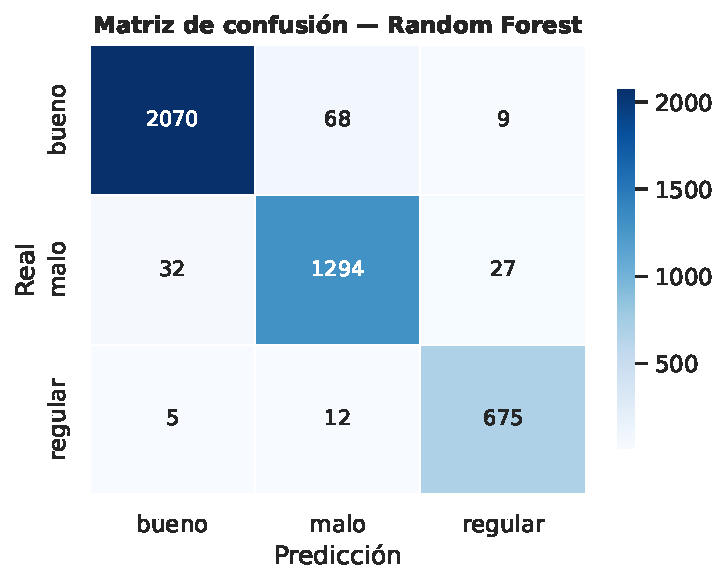
\includegraphics[width=\columnwidth]{fig_matriz_confusion_rf.pdf}
\caption{Matriz de confusión del modelo Random Forest en el conjunto de prueba.}
\label{fig:confusion_rf}
\end{figure}

\begin{figure}[h]
\centering
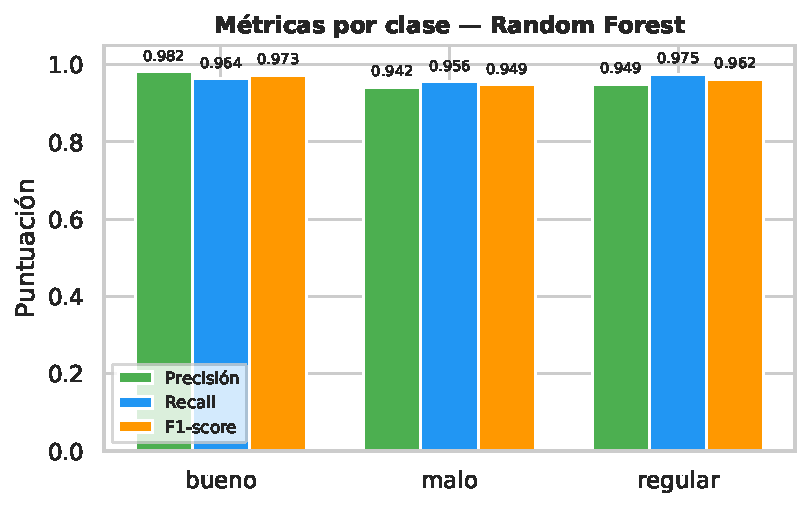
\includegraphics[width=\columnwidth]{fig_metricas_clase_rf.pdf}
\caption{Métricas de precisión, recall y F1 por clase para Random Forest.}
\label{fig:metricas_rf}
\end{figure}

\subsection{Red neuronal convolucional}
La CNN alcanzó tras 20 épocas:
\begin{itemize}
  \item Accuracy en prueba: 96.35\,\%
  \item Precisión macro: 0.9613
  \item Recall macro: 0.9601
  \item F1 macro: 0.9605
\end{itemize}

La Tabla~\ref{tab:comparativa} muestra las métricas por clase para el mejor modelo (Random Forest).

\begin{table}[h]
\centering
\caption{Métricas por clase — Random Forest.}
\label{tab:comparativa}
\begin{tabular}{lccc}
\toprule
Clase   & Precisión & Recall & F1 \\
\midrule
Bueno   & 0.98 & 0.96 & 0.97 \\
Malo    & 0.94 & 0.96 & 0.95 \\
Regular & 0.95 & 0.98 & 0.96 \\
\bottomrule
\end{tabular}
\end{table}

\subsection{Comparativa global}
La Tabla~\ref{tab:global} resume la comparación entre modelos.

\begin{table}[h]
\centering
\caption{Comparativa global de modelos.}
\label{tab:global}
\begin{tabular}{lcc}
\toprule
Modelo & F1 val. & F1 test \\
\midrule
Regresión Logística & 0.7363 & 0.7309 \\
Random Forest       & 0.9666 & 0.9615 \\
CNN                 & 0.9683   & 0.9605 \\
\bottomrule
\end{tabular}
\end{table}

\begin{figure}[h]
\centering
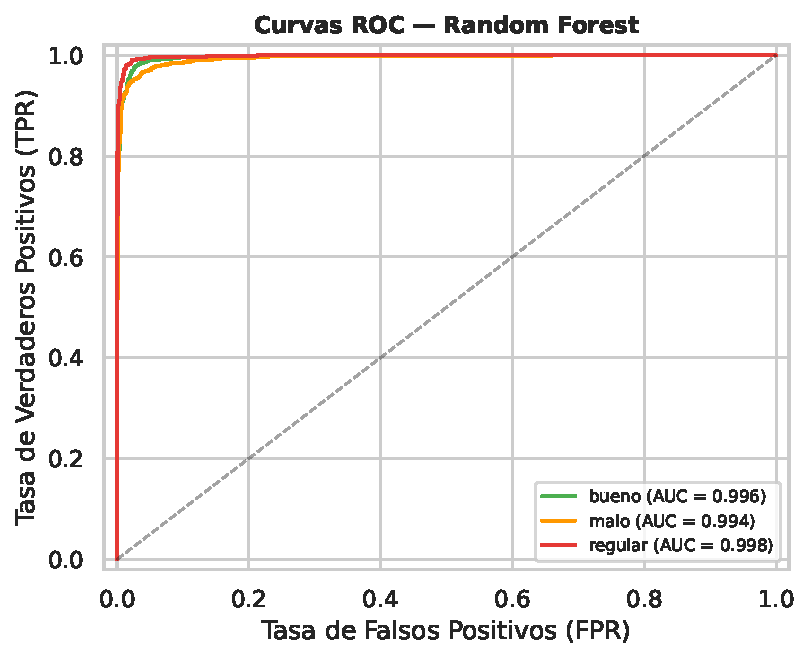
\includegraphics[width=\columnwidth]{fig_roc_rf.pdf}
\caption{Curvas ROC para cada clase — Random Forest.}
\label{fig:roc_rf}
\end{figure}

Ambos modelos (RF y CNN) cometieron 153 errores sobre 4\,192 imágenes de prueba (3.65\,\%). Los errores más comunes ocurrieron entre las clases \emph{malo} y \emph{regular} en frutas con daños parciales.

\subsection{Cobertura de imagen}
La cobertura estimada varió según la distancia de captura y el tamaño de la fruta, con una media del 66.5\,\% sobre el conjunto de datos (DE = 29.3\,\%). Este valor permite al usuario tener una noción del tamaño relativo del producto en el encuadre.

% ===========================================================================
% 7. ANÁLISIS DE RESULTADOS
% ===========================================================================
\section{Análisis de resultados}

\subsection{Desempeño de los modelos}
Random Forest y CNN presentan un desempeño casi idéntico (96.15\,\% vs 96.05\,\% de F1 macro), superando ampliamente a la regresión logística (73.63\,\%). Esta brecha de 23 puntos porcentuales merece un análisis cuidadoso.

La regresión logística asume que la frontera de decisión entre clases es lineal en el espacio de características. Para nuestro problema, esto implica que la diferencia entre una fruta \emph{buena} y una \emph{regular} debe ser separable mediante una combinación lineal de los 102 valores del histograma. Sin embargo, la realidad es más compleja: la presencia de una mancha pequeña puede ser irrelevante en una fruta (sigue siendo \emph{buena}) pero determinante en otra (la hace \emph{regular}); esta es una interacción no lineal que la regresión logística no puede capturar.

Random Forest, en cambio, modela estas interacciones de forma natural: un árbol puede dividir primero por el bin de rojo intenso (detectando fruta madura), luego por el bin de marrón (detectando podredumbre), y luego por la desviación estándar (detectando si el daño es localizado o generalizado). Esta capacidad de capturar relaciones jerárquicas y no lineales entre características es la razón principal por la que RF duplica efectivamente el desempeño de la línea base lineal.

La CNN, por su parte, aprende sus propias características visuales directamente de los píxeles, sin depender de histogramas precomputados. El hecho de que ambos modelos (RF y CNN) converjan al mismo nivel de accuracy (96.35\,\%) sugiere que ese es el techo práctico dado el nivel de subjetividad y ruido en las etiquetas del dataset.

\subsection{Generalización}
La diferencia entre el F1 de validación (0.9666) y el de prueba (0.9615) para RF es de solo 0.5 puntos porcentuales, lo que indica que no hay sobreajuste significativo. Además, el error OOB (\emph{out-of-bag}) estimado durante el entrenamiento fue de 3.8\,\%, consistente con el 3.65\,\% de error en prueba, confirmando que el modelo generaliza correctamente sin necesidad de validación cruzada adicional. La CNN muestra un comportamiento similar: las curvas de entrenamiento (accuracy y loss) convergen sin divergencia entre train y validación, y el F1 macro de prueba (0.9605) está alineado con el desempeño en validación durante el entrenamiento.

\subsection{Importancia de características}
Random Forest proporciona una medida de importancia para cada característica basada en la reducción de impureza (Gini) que produce al ser usada en las divisiones de los árboles. La Figura~\ref{fig:importancia} muestra las 15 características más influyentes.

Se observa que los \emph{histogramas de color} dominan el ranking: los bins de los canales rojo (C1), verde (C2) y azul (C3) aparecen repetidamente, junto con la media de cada canal. Esto tiene sentido físico: una fruta en mal estado tiende a oscurecerse o desarrollar tonos marrones (cambio en el canal rojo y verde), mientras que una fruta verde pero sana tiene picos diferentes en el histograma. La desviación estándar también es relevante porque captura la heterogeneidad del color: una mancha localizada aumenta la varianza cromática.

\begin{figure}[h]
\centering
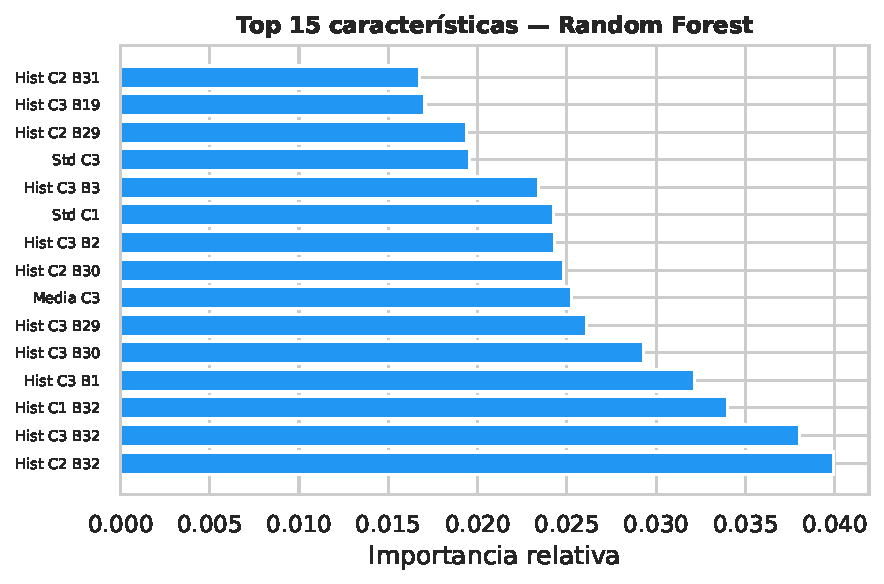
\includegraphics[width=\columnwidth]{fig_importancia_rf.pdf}
\caption{Las 15 características más importantes para el modelo Random Forest, basadas en histogramas de color RGB. Los bins de histograma de los canales rojo (C1), verde (C2) y azul (C3) dominan el ranking.}
\label{fig:importancia}
\end{figure}

\subsection{Análisis de errores}
El 3.65\,\% de errores se concentra en imágenes donde los defectos son sutiles o donde la iluminación y el fondo generan confusión. Las confusiones predominantes son entre \emph{malo} y \emph{regular}, que son las categorías más difíciles de diferenciar incluso para un humano.

\subsection{Comparación con la literatura}
Estudios similares reportan accuracy entre 90\,\% y 97\,\% para clasificación de calidad de frutas con CNN~\cite{lu2018quality, kamilaris2018deep}. Nuestros resultados (96.35\,\%) se encuentran en el rango superior, posiblemente debido a la calidad del dataset y la combinación de modelos.

\subsection{Aspectos éticos}
El sistema presenta sesgos inherentes al desbalanceo de clases: la clase \emph{regular} (16.5\,\% de los datos) tiene menor representación, aunque SMOTE mitigó este efecto. Es importante considerar que un sistema de este tipo podría ser utilizado para rechazar productos de pequeños agricultores si no se calibra adecuadamente con datos representativos de su contexto. La privacidad de las imágenes capturadas debe garantizarse mediante almacenamiento local y procesamiento sin transmisión a servidores externos.

\subsection{Impacto social y económico}
La implementación de sistemas automatizados de clasificación puede reducir el desperdicio de alimentos al detectar tempranamente productos en mal estado, estandarizar la calidad en la cadena de suministro y disminuir la dependencia de evaluadores humanos en tareas repetitivas. Sin embargo, su adopción debe considerar el costo de implementación y la capacitación necesaria para su uso en contextos agroindustriales de pequeña escala.

% ===========================================================================
% 8. CONCLUSIONES Y TRABAJO FUTURO
% ===========================================================================
\section{Conclusiones y trabajo futuro}

\subsection{Conclusiones}
Se desarrolló un sistema de clasificación de calidad de frutas con un desempeño superior al 96\,\% de accuracy, utilizando Random Forest y CNN. Ambos modelos son viables para despliegue, aunque RF ofrece la ventaja de un entrenamiento más rápido y menor consumo computacional. La interfaz Streamlit permite una interacción intuitiva y la estimación de cobertura proporciona información complementaria sobre el tamaño relativo. La metodología CRISP-DM guió el desarrollo de manera estructurada, desde la comprensión del negocio hasta el despliegue.

\subsection{Trabajo futuro}
Las siguientes líneas de mejora se identifican:
\begin{enumerate}
  \item Recolectar más imágenes de la clase \emph{regular} para reducir el desbalanceo.
  \item Implementar transferencia de aprendizaje con modelos pre-entrenados (ResNet, EfficientNet).
  \item Agregar estimación de tamaño absoluto mediante un objeto de referencia en la imagen.
  \item Desplegar el sistema en un dispositivo embebido (Raspberry Pi) para simulación de línea de empaque en tiempo real.
  \item Incorporar aumentación de datos durante el entrenamiento para mejorar la robustez ante variaciones de iluminación y fondo.
\end{enumerate}

% ===========================================================================
% 9. REFERENCIAS
% ===========================================================================
\bibliographystyle{IEEEtran}
\begin{thebibliography}{9}

\bibitem{kaggle_fruit}
R. Park, ``Fruit Quality Classification,'' Kaggle, 2024. [En línea]. Disponible: \url{https://www.kaggle.com/datasets/ryandpark/fruit-quality-classification}

\bibitem{fao_waste}
FAO, ``Global Food Losses and Food Waste,'' Organización de las Naciones Unidas para la Alimentación y la Agricultura, 2011.

\bibitem{breiman2001random}
L. Breiman, ``Random Forests,'' \textit{Machine Learning}, vol.~45, no.~1, pp.~5--32, 2001.

\bibitem{breiman1996bagging}
L. Breiman, ``Bagging Predictors,'' \textit{Machine Learning}, vol.~24, no.~2, pp.~123--140, 1996.

\bibitem{lecun2015deep}
Y. LeCun, Y. Bengio y G. Hinton, ``Deep learning,'' \textit{Nature}, vol.~521, pp.~436--444, 2015.

\bibitem{chawla2002smote}
N. V. Chawla, K. W. Bowyer, L. O. Hall y W. P. Kegelmeyer, ``SMOTE: Synthetic Minority Over-sampling Technique,'' \textit{Journal of Artificial Intelligence Research}, vol.~16, pp.~321--357, 2002.

\bibitem{canny1986computational}
J. Canny, ``A Computational Approach to Edge Detection,'' \textit{IEEE Trans. Pattern Analysis and Machine Intelligence}, vol.~8, no.~6, pp.~679--698, 1986.

\bibitem{lu2018quality}
S. Lu, Z. Lu, S. A. Arefin, ``Quality Classification of Fruits Using Computer Vision: A Review,'' \textit{Int. Journal of Agricultural and Biological Engineering}, vol.~11, no.~6, pp.~1--12, 2018.

\bibitem{kamilaris2018deep}
A. Kamilaris y F. X. Prenafeta-Boldú, ``Deep learning in agriculture: A survey,'' \textit{Computers and Electronics in Agriculture}, vol.~147, pp.~70--90, 2018.

\bibitem{grandini2020metrics}
M. Grandini, E. Bagli y G. Visani, ``Metrics for Multi-Class Classification: an Overview,'' \textit{arXiv preprint arXiv:2008.05756}, 2020.

\bibitem{histogram_features}
R. C. González y R. E. Woods, \textit{Digital Image Processing}, 4th ed. Pearson, 2018.

\end{thebibliography}

\end{document}
